\chapter{Diagrama de classes}
\addcontentsline{toc}{chapter}{Diagrama de classes}

Como podemos verificar no diagrama descrito na figura \ref{figure_diagrama_classe} as entidades do sistema consistem na medida, que é a informação que foi capturada pelo arduino, uma entidade abstrata que é entendida pelas classes concretas das medidas, temos também as entidades que representam o arduino, possuindo a localização do mesmo e o usuário, ambos extendendo da classe autentical.

\begin{figure}[H]
    \label{figure_diagrama_classe}
    \centering
    \caption{Diagrama de classes}
    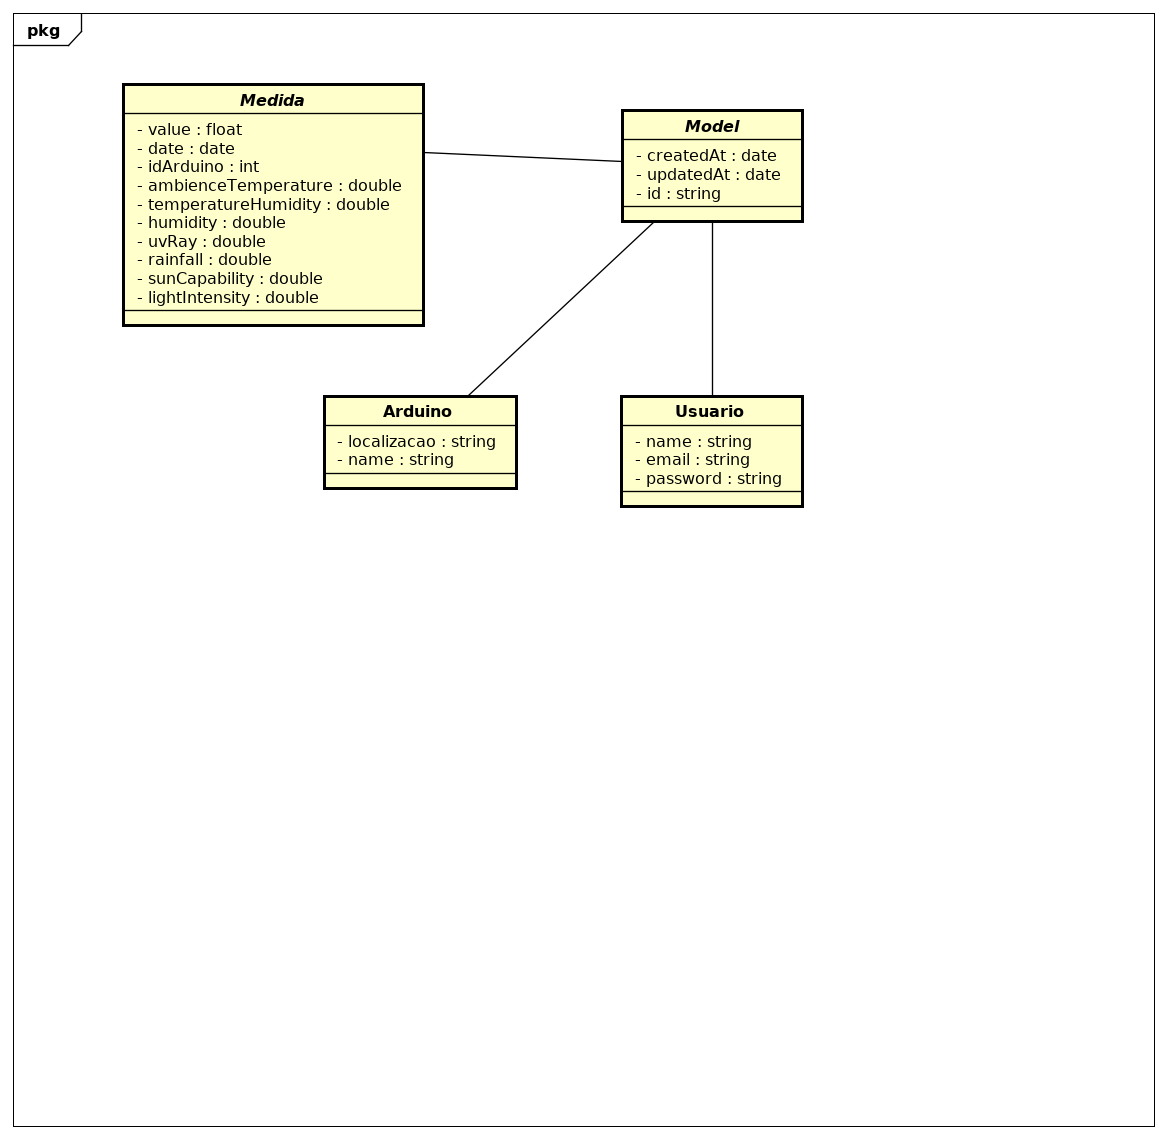
\includegraphics[scale=0.5]{diagrams/classe.png}
    \hfill
\end{figure}
